% TikZ代码:测试用例生成流程图
% 用于Design章节 - Parameter Space Exploration小节

\documentclass[tikz,border=10pt]{standalone}
\usepackage{tikz}
\usetikzlibrary{shapes,arrows,positioning,calc}

\begin{document}

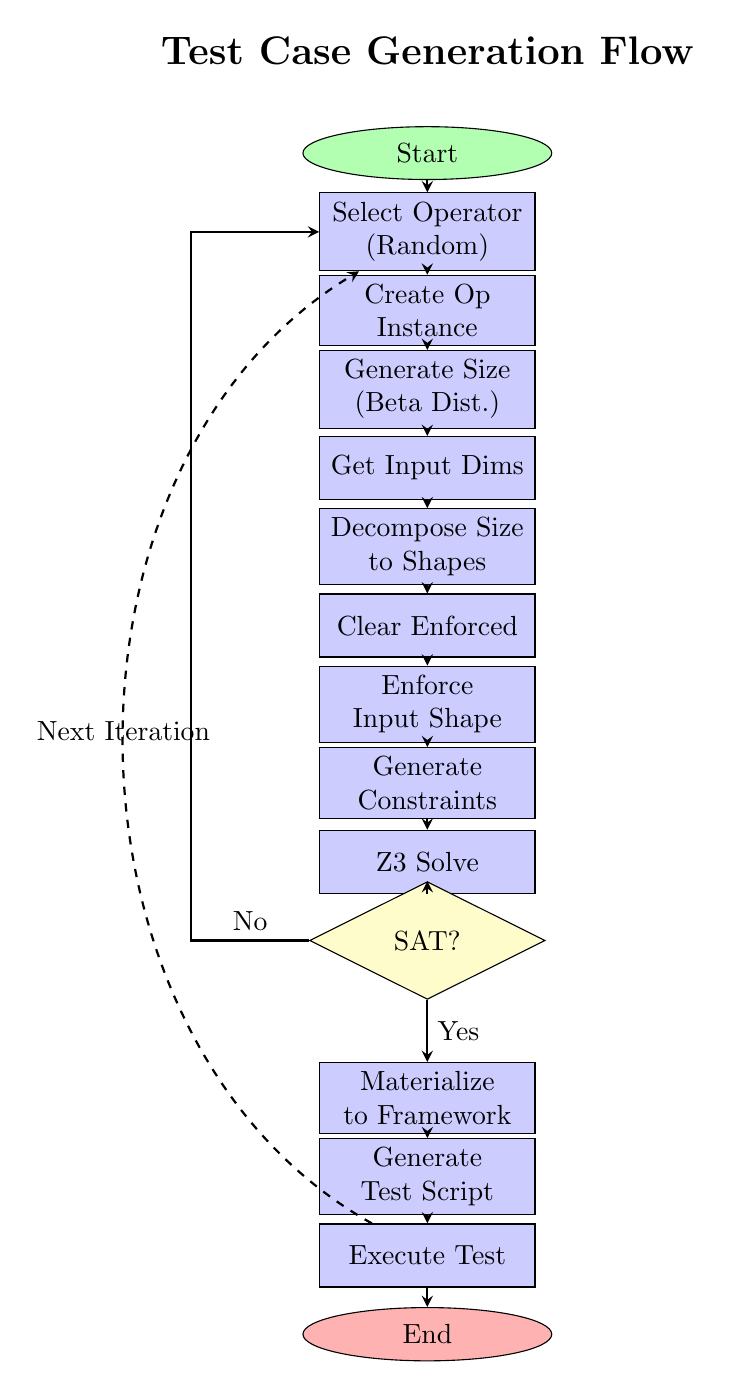
\begin{tikzpicture}[
    node distance=1cm,
    auto,
    start/.style={ellipse, draw, fill=green!30, text width=2cm, text centered},
    process/.style={rectangle, draw, fill=blue!20, text width=2.5cm, text centered, minimum height=0.8cm},
    decision/.style={diamond, draw, fill=yellow!20, text width=1.8cm, text centered, aspect=2},
    end/.style={ellipse, draw, fill=red!30, text width=2cm, text centered},
    arrow/.style={->, >=stealth, thick}
]

% 开始
\node[start] (start) {Start};

% 操作符选择
\node[process, below of=start] (select_op) {Select Operator \\ (Random)};
\node[process, below of=select_op] (create_op) {Create Op Instance};
\node[process, below of=create_op] (gen_size) {Generate Size \\ (Beta Dist.)};
\node[process, below of=gen_size] (get_dim) {Get Input Dims};

% 形状分解
\node[process, below of=get_dim] (decompose) {Decompose Size \\ to Shapes};
\node[process, below of=decompose] (clear) {Clear Enforced};
\node[process, below of=clear] (enforce) {Enforce Input Shape};

% 约束生成和求解
\node[process, below of=enforce] (gen_const) {Generate Constraints};
\node[process, below of=gen_const] (z3_solve) {Z3 Solve};
\node[decision, below of=z3_solve] (check_sat) {SAT?};

% 框架转换
\node[process, below of=check_sat, yshift=-1cm] (materialize) {Materialize \\ to Framework};
\node[process, below of=materialize] (gen_script) {Generate Test Script};
\node[process, below of=gen_script] (execute) {Execute Test};

% 结束
\node[end, below of=execute] (end) {End};

% 连接线
\draw[arrow] (start) -- (select_op);
\draw[arrow] (select_op) -- (create_op);
\draw[arrow] (create_op) -- (gen_size);
\draw[arrow] (gen_size) -- (get_dim);
\draw[arrow] (get_dim) -- (decompose);
\draw[arrow] (decompose) -- (clear);
\draw[arrow] (clear) -- (enforce);
\draw[arrow] (enforce) -- (gen_const);
\draw[arrow] (gen_const) -- (z3_solve);
\draw[arrow] (z3_solve) -- (check_sat);
\draw[arrow] (check_sat) -- node[right] {Yes} (materialize);
\draw[arrow] (check_sat) -- node[above, sloped] {No} ++(-3,0) |- (select_op);
\draw[arrow] (materialize) -- (gen_script);
\draw[arrow] (gen_script) -- (execute);
\draw[arrow] (execute) -- (end);

% 循环箭头
\draw[arrow, dashed, bend left=60] (execute) to node[above] {Next Iteration} (select_op);

% 标题
\node[above of=start, yshift=0.3cm, font=\Large\bfseries] {Test Case Generation Flow};

\end{tikzpicture}

\end{document}

